\documentclass[runningheads]{llncs}

% ---------------------------------------------------------------
% Include basic ECCV package
 
% TODO REVIEW: Insert your submission number below by replacing '*****'
% TODO FINAL: Comment out the following line for the camera-ready version
\usepackage[review,year=2026,ID=12703]{eccv}
% TODO FINAL: Un-comment the following line for the camera-ready version
% \usepackage{eccv}

% OPTIONAL: Un-comment the following line for a version which is easier to read
% on small portrait-orientation screens (e.g., mobile phones, or beside other windows)
%\usepackage[mobile]{eccv}


% ---------------------------------------------------------------
% Other packages

% Commonly used abbreviations (\eg, \ie, \etc, \cf, \etal, etc.)
\usepackage{eccvabbrv}

% Include other packages here, before hyperref.
\usepackage{graphicx}
\usepackage{booktabs}

% The "axessiblity" package can be found at: https://ctan.org/pkg/axessibility?lang=en
\usepackage[accsupp]{axessibility}  % Improves PDF readability for those with disabilities.


% ---------------------------------------------------------------
% Hyperref package

% It is strongly recommended to use hyperref, especially for the review version.
% Please disable hyperref *only* if you encounter grave issues.
% hyperref with option pagebackref eases the reviewers' job, but should be disabled for the final version.
%
% If you comment hyperref and then uncomment it, you should delete
% main.aux before re-running LaTeX.
% (Or just hit 'q' on the first LaTeX run, let it finish, and you
%  should be clear).

% TODO FINAL: Comment out the following line for the camera-ready version
%\usepackage[pagebackref,breaklinks,colorlinks,citecolor=eccvblue]{hyperref}
% TODO FINAL: Un-comment the following line for the camera-ready version
\usepackage{hyperref}

\usepackage{xcolor}
% Support for ORCID icon
\usepackage{orcidlink}

%% Additional packet
\usepackage{newfloat}
\usepackage{listings}
\usepackage{multirow}
\usepackage{algorithm}
\usepackage{pgfplots}
\usepackage{newfloat}
\usepackage{algorithmicx}
\usepackage{algorithm}
\usepackage{algpseudocode}
\pgfplotsset{compat=1.17}
\usepgfplotslibrary{colorbrewer} % For professional academic colors

\definecolor{duong}{rgb}{91,10,145}
\begin{document}

% ---------------------------------------------------------------
% TODO REVIEW: Replace with your title
\title{H-SFP: Hierarchical Federated Learning with Decoupled Split-Model Prototyping}
% \title{H-SFP: Computation and communication-efficient Hierarchical Federated Learning with Split-Aware Distributional Prototyping}
% \title{H-SFP: Decoupled Hierarchical Federated Learning via Distributional Prototyping}
% \title{H-SFP: Lightweight Federated Learning via HiMimi Zhang erarchical Split Prototyping} 

% TODO REVIEW: If the paper title is too long for the running head, you can set
% an abbreviated paper title here. If not, comment out.
% \titlerunning{Hierarchical split-federated prototyping}

% TODO FINAL: Replace with your author list. 
% Include the authors' OCRID for the camera-ready version, if at all possible.
\author{First Author\inst{1}\orcidlink{0000-1111-2222-3333} \and
Second Author\inst{2,3}\orcidlink{1111-2222-3333-4444} \and
Third Author\inst{3}\orcidlink{2222--3333-4444-5555}}

% TODO FINAL: Replace with an abbreviated list of authors.
\authorrunning{F.~Author et al.}
% First names are abbreviated in the running head.
% If there are more than two authors, 'et al.' is used.

% TODO FINAL: Replace with your institution list.
\institute{Princeton University, Princeton NJ 08544, USA \and
Springer Heidelberg, Tiergartenstr.~17, 69121 Heidelberg, Germany
\email{lncs@springer.com}\\
\url{http://www.springer.com/gp/computer-science/lncs} \and
ABC Institute, Rupert-Karls-University Heidelberg, Heidelberg, Germany\\
\email{\{abc,lncs\}@uni-heidelberg.de}}

\maketitle
\begin{abstract}
    Federated learning (FL) enables collaborative model training without sharing raw data, but practical deployments must balance statistical heterogeneity, resource-constrained clients, and communication efficiency. While conventional FL requires clients to train full models locally, split federated learning (SFL) reduces client-side computation by partitioning models across tiers, at the cost of transmitting high-dimensional activations and gradients during training. We propose Hierarchical Split-Federated Prototyping (H-SFP), a communication-efficient framework for hierarchical cloud–edge–client environments. Instead of exchanging sample-level activations or gradients, H-SFP communicates compact class-wise feature statistics and uses them to synthesize representative feature distributions at upper tiers. This statistical prototyping mechanism enables independent training of model segments while preserving the computational advantages of split-model execution and substantially reducing synchronization and communication overhead.
    A key finding of this work is that lightweight first- and second-order feature statistics are sufficient to support hierarchical split-model training, providing an effective communication interface without requiring sample-level feature exchange. We analyze the communication properties and stability of the proposed statistical interface under hierarchical aggregation. Extensive experiments on CIFAR-10/100, HAM10000, ImageNet-1K, and ISIC-2018 demonstrate that H-SFP remains robust under heterogeneous data distributions while reducing communication overhead by up to two orders of magnitude compared with federated and split-learning baselines.
\keywords{Federated Learning, Hierarchical Federated Learning, Split Federated Learning, Feature Prototyping, Communication Efficiency}
\end{abstract}


    
\section{Introduction}\label{sec:intro}

Federated learning (FL) \cite{pmlr-v54-mcmahan17a} enables collaborative model training across distributed clients without exchanging raw data, making it a promising paradigm for privacy-sensitive visual learning. Despite this advantage, practical FL deployments must balance three competing factors: statistical heterogeneity across clients \cite{tan2022fedproto,10660707,nguyen2026towards}, limited computational resources on edge devices \cite{MAL-083,11180918}, and communication efficiency in large-scale distributed systems \cite{nguyen2022hcfl,nguyen2025federated}. Conventional FL methods typically require each client to train the full model locally, which can be prohibitively expensive for resource-constrained devices \cite{9760729,9084352,dai2023tacklingFedProx}.

Split federated learning (SFL) addresses this limitation by partitioning model execution across clients and servers \cite{thapa2022splitfed}. By assigning only shallow network layers to clients, SFL reduces client-side computation and memory requirements \cite{GUPTA20181,vepakomma2019split}. Hierarchical SFL further extends this idea to cloud--edge--client systems, where edge servers provide intermediate computation and aggregation. However, existing SFL and hierarchical SFL (HSFL) frameworks usually rely on transmitting intermediate activations during the forward pass and propagating gradients during backpropagation \cite{11091500,zhang2025amperecommunicationefficienthighaccuracysplit,qiu2023evaluating,wang2025towards}. This sample-level communication creates substantial bandwidth consumption, introduces synchronization dependencies across tiers, and couples the optimization of client, edge, and cloud components \cite{10980018,quan2023hiersfl}. These challenges become more pronounced as models, client populations, and data heterogeneity increase.

In this work, we revisit the communication interface of hierarchical split learning. Instead of exchanging sample-level activations and gradients, we ask whether compact class-level feature statistics can provide sufficient information for training upper model components. Our key observation is that first- and second-order statistics of client-side feature embeddings can preserve useful class-level semantic structure while requiring much less communication than activation-level exchange. This motivates a statistical feature-prototyping mechanism, in which upper tiers synthesize representative feature distributions from compact summaries rather than relying on direct cross-tier backpropagation.

Based on this principle, we propose \textbf{Hierarchical Split-Federated Prototyping (H-SFP)}, a communication-efficient framework for cloud--edge--client learning. In H-SFP, clients execute lightweight feature extractors and transmit only class-wise feature statistics to nearby edge servers. Edge servers aggregate these statistics, synthesize representative feature samples, and train intermediate model components. The cloud tier further aggregates distribution-level summaries to train task-specific layers. By replacing activation and gradient exchange with statistical feature prototyping, H-SFP preserves the computational advantage of split-model execution while decoupling optimization across hierarchical tiers and reducing communication overhead.

The main finding of this work is that compact statistical summaries can serve as an effective communication interface for HSFL. Although H-SFP does not transmit sample-level activations or gradients across tiers, it maintains strong performance under heterogeneous data distributions while substantially reducing communication cost. Our contributions are summarized as follows:
\begin{itemize}
\item We propose H-SFP, a communication-efficient hierarchical split-federated framework that replaces sample-level activation and gradient exchange with compact class-wise feature statistics.

\item We introduce a statistical feature-prototyping mechanism that enables the edge and cloud tiers to synthesize representative feature distributions and to train upper-model components without cross-tier backpropagation.

\item We provide theoretical analysis of prototype-induced distribution shift and the stability of statistical feature representations in hierarchical setups.

\item We conduct experiments on image classification and medical image segmentation benchmarks, demonstrating robust performance under heterogeneous data distributions with substantially reduced communication overhead.
\end{itemize}

\section{Background and Related Works}
\label{sec:related_works}
Our work lies at the intersection of research directions addressing the inherent trilemma of FL: statistical heterogeneity, system heterogeneity, and communication bottlenecks. The first category, standard FL, aims to collaboratively train global models without centralizing raw data. Fundamental algorithms like FedAvg~\cite{pmlr-v54-mcmahan17a} often suffer from severe ``client drift'' due to non-IID data distributions. To mitigate this, traditional solutions rely on regularization mechanisms, such as proximal terms in FedProx~\cite{dai2023tacklingFedProx}, or momentum-based optimization~\cite{cheng2024momentumbenefits, zaccone2025communication}. To address variable local work across heterogeneous clients, FedNova~\cite{10.5555/3495724.3496362} normalizes client updates before aggregation. However, a critical limitation of these frameworks is that they inherently assume clients possess the computational capacity to train and evaluate full models locally. This assumption exacerbates system heterogeneity and excludes resource-constrained edge devices from participating.

To alleviate these client-side computational constraints, SFL partitions the model and offloads heavy upper layers to the server. SplitFed~\cite{thapa2022splitfed} was introduced to parallelize client updates, resolving the sequential training bottlenecks of early split learning. This literature has expanded to address computational diversity and scale through HeteroSFL paradigms that build on sub-model deployments such as HeteroFL~\cite{diao2021heterofl} and Hierarchical SFL (HSFL)~\cite{rana2022hierarchical,9148862,9488756}, which introduce edge servers for intermediate synchronization. Despite these topological advancements, these frameworks suffer from limitations. They require the continuous transmission of high-dimensional activations during the forward pass and the subsequent return of gradients during the backward pass. This bidirectional dependency introduces synchronization overhead, exacerbates communication bottlenecks, and creates new computational bottlenecks on the server~\cite{10980018}.

As an alternative to raw gradient and activation communication, the third category explores generative and prototype-based FL. Methods such as Federated Knowledge Distillation (FedDF~\cite{lin2020ensemble}) and data-free Generative FL (FedGen~\cite{venkateswaran2023fedgen}) address both communication overhead and non-IID challenges but typically require training computationally expensive generators, such as GANs, at the server. Conversely, prototype-based FL, such as FedProto~\cite{tan2022fedproto} or FOUL \cite{nguyen2026computation}, exchanges lightweight class prototypes instead of gradients or heavy activations. A major limitation of prototype methods, however, is that they primarily utilize these prototypes as client-side regularization terms to align local feature spaces. Because they are not used to synthesize actual training data, these methods can still suffer from prototype drift under extreme heterogeneity~\cite{bensiah2025feddpa, zhang2020personalized}.

\textcolor{black}{H-SFP complements these resource-efficient and decoupled learning approaches. PriSM~\cite{niu2023overcoming} reduces client computation by sampling principal kernels to construct lightweight sub-models, while Delta~\cite{10655220} studies asymmetric private/public computation flows with explicit privacy mechanisms. In contrast, H-SFP focuses on the HSFL setting, where clients, edge servers, and the cloud train different model segments. Its main design choice is a statistic-based cross-tier interface: upper tiers receive class-wise feature moments rather than sample-wise activations, gradients, full model updates, or learned generators. This makes H-SFP particularly suitable for hierarchical deployments.}

Existing frameworks preserve a shared end-to-end optimization graph across tiers. Even when activations or prototypes are transmitted rather than full models, the upper and lower tiers remain coupled via cross-tier gradient propagation or parameter synchronization. This architectural dependency forces all components to participate in a single distributed optimization process, making communication and statistical drift intrinsically entangled.
In contrast, H-SFP departs from this paradigm by severing the optimization graph across tiers. \textcolor{black}{Rather than coordinating updates through sample-wise gradients or activations, H-SFP performs tier-wise optimization over synthesized feature distributions derived from aggregated statistical moments. This design provides a lightweight communication interface between client, edge, and cloud tiers while preserving the practical advantage of split-model execution on resource-constrained clients.}
A detailed comparison between approaches is shown in the Appendix~A.

\section{The Proposed H-SFP Framework}
\label{sec:methodology}
\begin{figure}[ht]
    \centering
    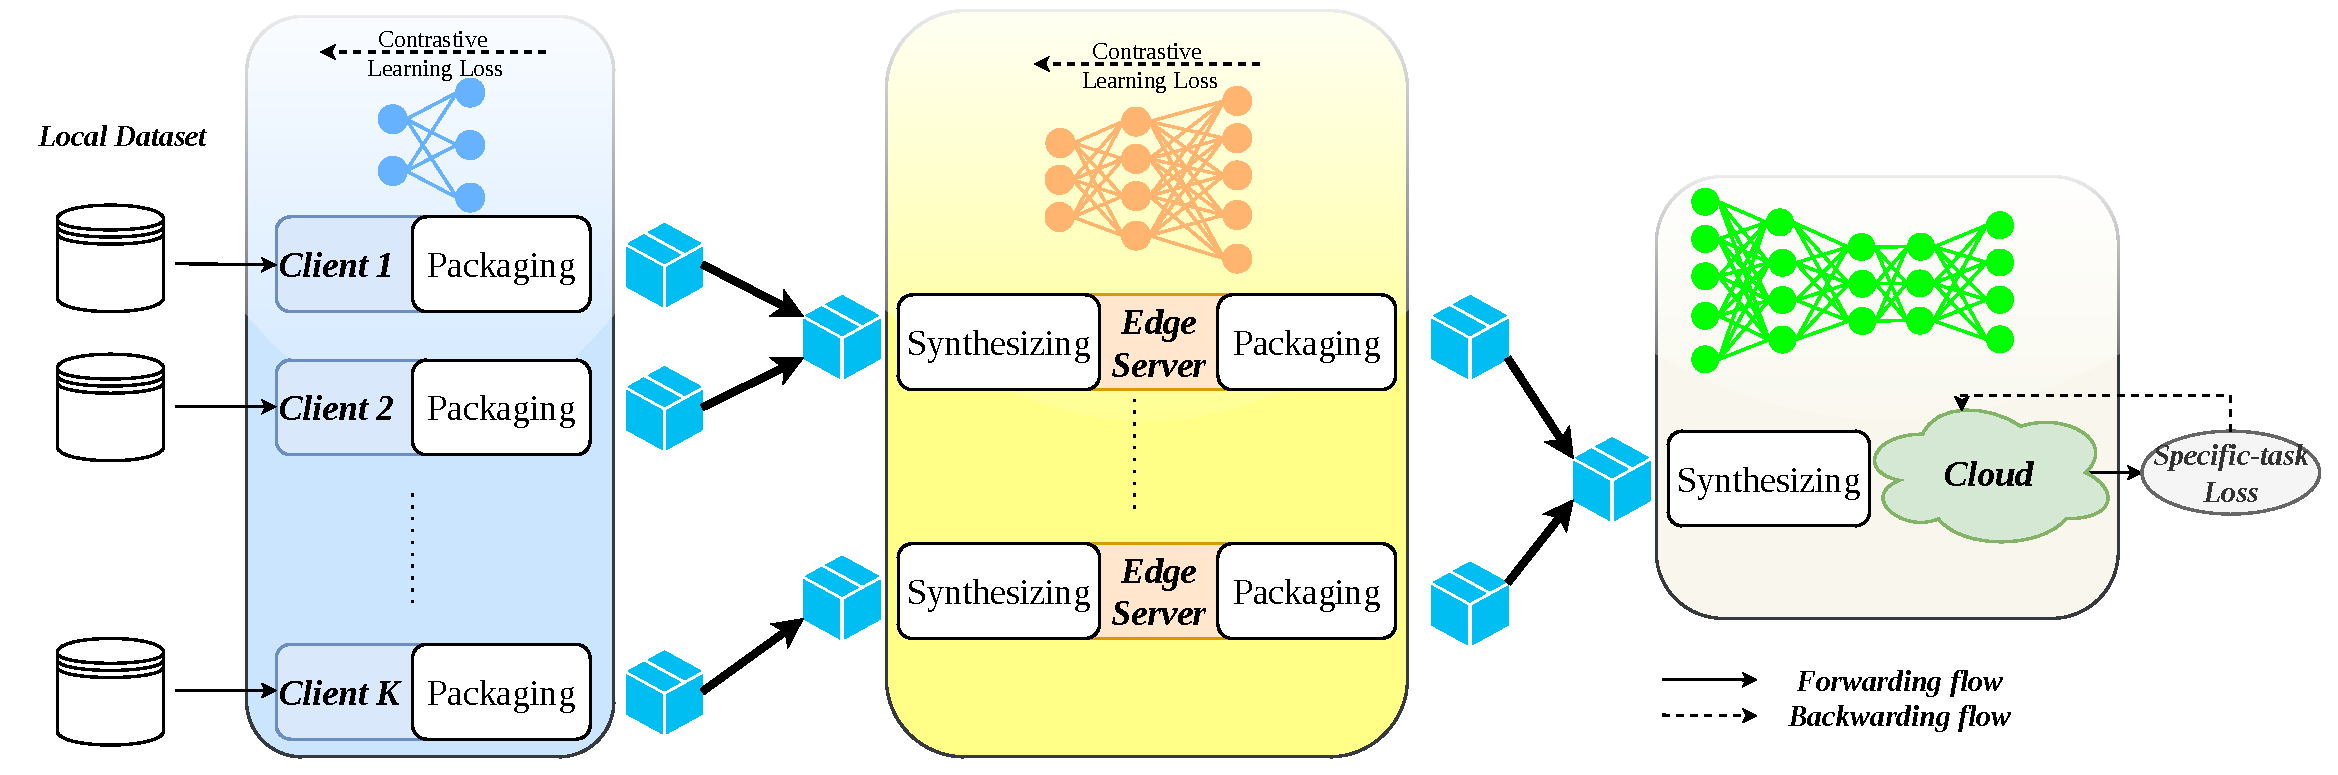
\includegraphics[width=\linewidth]{
    Figures/method-2.pdf}
    \caption{The H-SFP architecture and data flow. Clients communicate class-wise feature statistics instead of sample-level activations and gradients. Edge and cloud tiers iteratively aggregate statistics, synthesize feature distributions, and train their assigned model components.}
    \label{fig:method-p2}
\end{figure}
\begin{figure}[t]
    \centering
    \begin{subfigure}{0.44\linewidth}
        \centering
        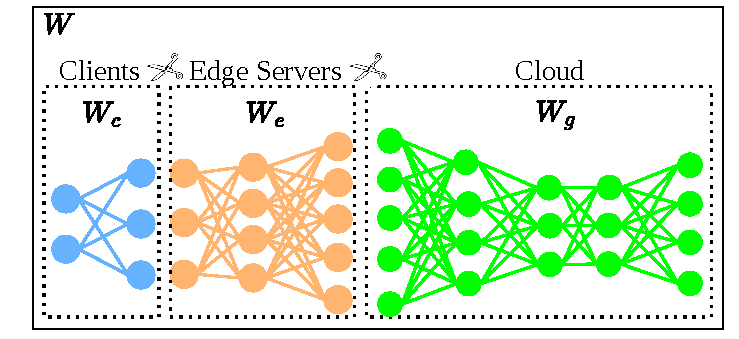
\includegraphics[width=\linewidth]{Figures/method-3.pdf}
        \caption{Hierarchical Model Partitioning.}
        \label{fig:method-p3}
    \end{subfigure}
    \hfill
    \begin{subfigure}{0.54\linewidth}
        \centering
        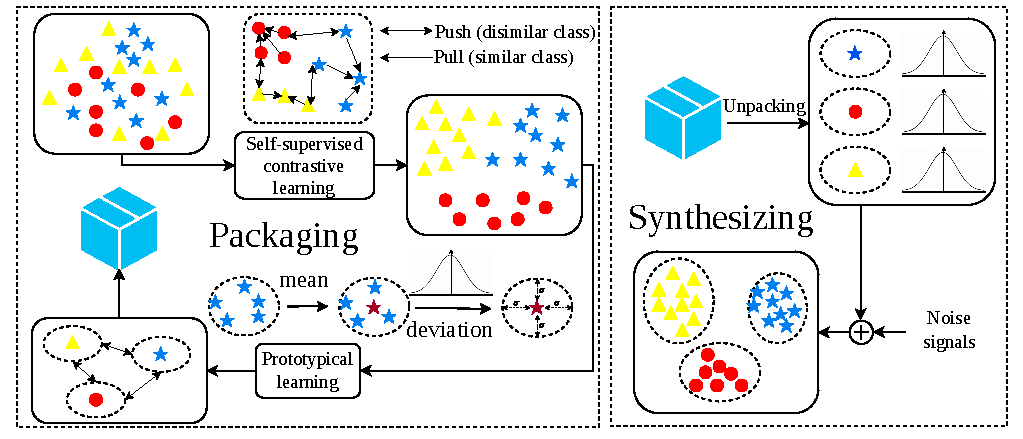
\includegraphics[width=\linewidth]{Figures/method-1.pdf}
        \caption{Generative Prototyping.}
        \label{fig:method-p1}
    \end{subfigure}
    \caption{The proposed H-SFP Framework. (a) Model partitioning ($W_c, W_e, W_g$) offloads computational burden from the clients. (b) The core generative prototyping mechanism, where self-supervised contrastive learning at the client level enables the compression of representations into lightweight statistical moments ($\mu$, $\sigma$).}
    \label{fig:h_sfp_framework_combined}
\end{figure}
We propose H-SFP, which replaces cross-tier backpropagation with statistic-based feature synthesis. Each tier trains its assigned model part locally, packages its learned feature distribution into lightweight class-wise statistics, and transmits only these statistics upward. The following subsections describe the system architecture, prototype packaging and synthesis, and the resulting communication behavior. 
Concrete algorithms for each tier are provided in the Appendix~B.

\subsection{System Architecture and Motivation}
\label{subsec:system_model}
We consider a three-tier ``cloud-edge-client'' framework shown in~\Cref{fig:method-p2}, comprising a global cloud server, $M$ edge servers, and $K$ clients partitioned into $M$ disjoint clusters $\{\mathcal{C}_m\}_{m=1}^M$. This framework directly addresses the scalability bottleneck of centralized FL by allowing edge servers to perform intermediate aggregations. In real-world deployments, this partitioning would be determined by physical proximity or by network latency pinging. However, for our empirical evaluation, we deliberately adopt a random assignment strategy. This represents a strict, unoptimized baseline, demonstrating that H-SFP's generative aggregation can successfully stabilize distributions and mitigate client drift even without the benefit of a geographically optimized or clustered network topology.

To solve resource-constrained clients, H-SFP adopts a split-learning architecture. As illustrated in \Cref{fig:method-p3}, the global model $W$ is partitioned into three components: a lightweight client-side feature extractor $W_c$, an intermediate edge-side model $W_e$, and a cloud-side task model $W_g$. This reduces the computational and memory burden on clients by offloading deeper network layers to upper tiers. However, conventional split federated learning requires continuous transmission of intermediate activations and gradients to maintain end-to-end optimization, leading to substantial communication and synchronization overhead.

H-SFP resolves this by replacing backpropagation with a feed-forward, multi-tier generative prototyping mechanism (\Cref{fig:method-p1}). By transmitting lightweight statistics rather than raw activations, we completely decouple the network segments, enabling communication-efficient and asynchronous training. Additionally, the precise cut points are treated as hyperparameters determined by the target device's memory constraints. For instance, clients may only compute the first residual block of a ResNet architecture, offloading the deeper, computationally expensive blocks to the edge and cloud tiers.

\subsection{Multi-tier Self-Learning} 
\label{sec:multi_tier_learning}
    
The first tier of learning occurs on resource-constrained clients. Each client $k$ trains its local extractor \textcolor{black}{$W_{c,k}$} using its private data $\mathcal{D}_k$. The objective $\mathcal{L}_k(W_{c,k})$ is to learn a robust representation space using the self-supervised NT-Xent contrastive loss \cite{chen2020simple}. For a batch $B$, let $z_i = W_{c,k}(x_i)$ where $x_i \in D_k$:
\begin{equation}
    \label{eq:supcon}
    \mathcal{L}_{k}(W_{c,k})= \mathcal{L}_{\text{con}, k} = \sum_{i\in B}\frac{-1}{|P(i)|}\sum_{p\in P(i)}\log\frac{\exp(z_{i}\cdot z_{p}/\tau)}{\sum_{a\in A(i)}\
    exp(z_{i}\cdot z_{a}/\tau)}
\end{equation}
where $A(i)$ is the set of other samples in the batch, $P(i)$ contains positive samples sharing the same class label as $i$, and $\tau$ is a temperature scalar. After training, the client distills its feature space into class-conditional statistics.
At the second tier, the edge server $m$ operates without access to real data. It aggregates the statistics $\{\mu_k, \sigma_k\}$ from its client cluster $\mathcal{C}_m$ to form a stable distribution $(\mu_m, \sigma_m)$. The edge server $m$ unpacks these statistics to synthesize a new feature dataset, $D^{syn}_m$, which serves as the input for the edge-side part $W_{e,m}$. $W_{e,m}$ is trained using the same contrastive objective on its own outputs, $\mathcal{L}_m(W_{e,m}) = \mathcal{L}_{\text{con}, m}(W_e(D_{syn}^{\text{edge}}))$. Enforcing consistency across tiers ensures that $W_e$ learns relative structural relationships rather than overfitting to synthetic noise.

Finally, the cloud tier aggregates the class-conditional feature statistics from all $M$ edge servers to form a global synthetic dataset, $D_{\text{syn}}^{\text{global}}$. The aggregated means and standard deviations are used to sample representative feature embeddings for each class. The task-specific part $W_g$ is then trained on this synthesized dataset using the standard supervised loss $\mathcal{L}_g(W_g) = \mathcal{L}_{\text{task}}\big(W_g(D_{syn}^{\text{global}})\big)$.

\subsection{Dual-Timescale Transmission and Augmentation}
\label{sec:transmission_augmentation}
Our communication mechanism operates on a dual-timescale to balance efficiency with long-term stability. At the fast timescale, clients transmit only their class-wise prototype statistics, including the local $\mu_{k}^{(j)}$ and $\sigma_{k}^{(j)}$ of class $j$:
\begin{equation}
    \mu_k^{(j)} = \frac{1}{|\mathcal{D}_k^{(j)}|} \sum_{x_i \in \mathcal{D}_k^{(j)}} W_{c,k}(x_i), \quad
    \sigma_k^{(j)} = \sqrt{\frac{1}{|\mathcal{D}_k^{(j)}|} \sum_{x_i \in \mathcal{D}_k^{(j)}} (W_{c,k}(x_i) - \mu_k^{(j)})^2}.
    \label{mean_std_client}
\end{equation}
This drastically reduces overhead to $O(J_k \times d_c)$ per client, where $J_k$ is the class count and $d_c$ the feature dimension. Infrequently (slow timescale interval $I_c$), a standard model averaging of $W_{c,k}$ occurs to correct long-term client drift. 

Upon receiving \textcolor{black}{($\mu_k$, $\sigma_k$)}, the edge server synthesizes features $z_{syn}$ for class $j$ by sampling from a multivariate Gaussian as in \cite{9578909,Nguyen_2026_CVPR} as follows:
\begin{equation}
    \label{eq:synthesis}
    z_{syn} \sim \mathcal{N}\big(\mu_m^{(j)}, \text{diag}(\sigma_m^{(j)} + \epsilon)^2\big)
\end{equation}
where $\text{diag}(\cdot)$ creates a diagonal covariance matrix and $\epsilon$ ensures numerical stability. We intentionally restrict the synthesis to a diagonal covariance matrix to achieve an optimal trade-off. Transmitting a full covariance matrix would increase the communication cost to $O(d_c^2)$, recreating the SL bottleneck. However, our ablation studies in \Cref{sec:ablation} confirm that transmitting per-dimension variance ($\sigma$) rather than just the mean ($\mu$) is critical for capturing the elliptical boundaries of feature clusters. Unlike SFL, which transmits exact, invertible activation maps for every sample, H-SFP transmits aggregated, class-wise statistics that obfuscate individual features, serving as a natural defense against feature-space inversion attacks while remaining semantically rich.

\subsection{Theoretical Justification: Information Preservation}
\label{sec:mmd_theory}
    
A fundamental concern with generative prototyping is the potential loss of high-rank structural information when replacing raw activations with $(\mu, \sigma)$. We theoretically bound this distribution shift between the true client representations $H_{true}$ and the edge-synthesized features $\hat{H}_{gen}$ using Maximum Mean Discrepancy (MMD). Let $\mathcal{X}$ be the feature space defined by $W_c$. Given a characteristic kernel $k: \mathcal{X} \times \mathcal{X} \rightarrow \mathbb{R}$ mapping to a Reproducing Kernel Hilbert Space (RKHS), the empirical MMD between the true feature distribution $\mathbb{P}$ and the synthesized Gaussian distribution $\mathbb{Q}$ is bounded by: 
\begin{equation}
\label{eq:mmd_bound}
\text{MMD}^2(\mathbb{P}, \mathbb{Q}) = \mathbb{E}_{x, x' \sim \mathbb{P}}[k(x, x')] + \mathbb{E}_{y, y' \sim \mathbb{Q}}[k(y, y')] - 2\mathbb{E}_{x \sim \mathbb{P}, y \sim \mathbb{Q}}[k(x, y)].
\end{equation}

To ensure $\text{MMD}^2(\mathbb{P}, \mathbb{Q}) \to 0$ and that the synthesized geometry preserves the semantic manifold, we introduce a statistical constraint on the feature extractor. 

\noindent\textbf{Assumption 1 (Feature-Space Lipschitz Continuity):} There exists a constant $L_{stat} > 0$ such that for any two data samples $x_1, x_2$, the divergence of their generated prototype statistics is bounded by the input space distance:
\begin{equation}
\label{eq:lipschitz}
||\mu(x_1) - \mu(x_2)||_2 + ||\sigma(x_1) - \sigma(x_2)||_2 \leq L_{stat} ||x_1 - x_2||_2.
\end{equation}
By enforcing Assumption 1 during local client updates via the contrastive loss, the divergence between the actual and synthesized manifolds remains strictly bounded across aggregation rounds, preventing information loss.

\subsection{Asymptotic Convergence Analysis}
\label{sec_convergence_analysis}

Establishing end-to-end convergence guarantees for the H-SFP topology requires departing from standard federated optimization proofs. Because our framework decouples the computational tiers, optimization at the upper tiers is performed over a dynamically shifting probability measure space parameterized by the tier below. To bound this shifting measure, we adopt standard stochastic non-convex assumptions along with a novel measure-theoretic constraint.

\noindent\textit{Assumption 2 (Measure Theoretic Lipschitz Continuity).} Let $\mathcal{P}(\mathcal{Z})$ denote the space of synthesized prototype measures. The expected loss functional $\mathcal{L}$ is $L_{m}$ Lipschitz continuous with respect to the Wasserstein 2 distance $\mathcal{W}_2$ between generated distributions $\mathbb{Q}_1, \mathbb{Q}_2 \in \mathcal{P}(\mathcal{Z})$:
\begin{equation}
|\mathbb{E}_{z \sim \mathbb{Q}_1}[\mathcal{L}(W; z)] - \mathbb{E}_{z \sim \mathbb{Q}_2}[\mathcal{L}(W; z)]| \le L_{m} \cdot \mathcal{W}_2(\mathbb{Q}_1, \mathbb{Q}_2).
\end{equation}

\noindent\textit{Assumption 3 (Bounded Variances and Second Moments).} The variance and second moments of stochastic gradients for each layer $l$ have upper bounds, denoted by $\sigma_l^2$ and $G_l^2$, respectively.
Operating under these constraints, we formally establish the global convergence of the decoupled architecture. The rigorous measure-theoretic derivation is deferred to the Appendix~C.

\noindent\textit{Theorem 1 (Asymptotic Convergence of H-SFP).} Under standard non-convex assumptions and Assumptions 2 and 3, the decoupled parameters asymptotically converge to a bounded stationary neighborhood. Specifically, for the global classifier $W$ optimized over $R$ total communication rounds with learning rate $\eta$, local aggregation intervals $I_m$, and layer split boundaries $L_m$, the expected gradient norm satisfies
\begin{multline}
\frac{1}{R}\sum_{t=1}^{R}\mathbb{E}[||\nabla \mathcal{L}(\overline{W}^{t-1})||_2^2] \le \frac{2\Delta}{\eta R} + \frac{L\eta\sum_{l=1}^{L_{\mathrm total}} \sigma_l^2}{N} \\ + 4L^2\eta^2\sum_{m=1}^{M-1}\left(\mathbb{I}_{\{I_m>1\}}I_m^2\sum_{l=L_{m-1}+1}^{L_m} G_l^2\right)
\end{multline}
where $\Delta = \mathcal{L}(\overline{W}^0) - \mathcal{L}^*$, and $\mathbb{I}_{\{\cdot\}}$ is the indicator function.

\noindent\textit{Proof Sketch (Hierarchical Measure Stabilization).} The proof proceeds inductively across the hierarchy. The induction initiates at the client tier, where the local extractors converge modulo standard SGD dynamics. The divergence between the aggregated sub-model and local sub-models is strictly bounded by the aggregation interval $I_m$ and the second moments $G_l^2$. Given $L_f$ Lipschitz embeddings, the sequence of client output measures stabilizes, driving the expected parametric shift to zero. As the edge model $W_e$ optimizes over the synthesized measure $\mathbb{Q}_{e}^t$, its temporal update incurs a stochastic drift bounded by $\delta_m^t = L_{m} \cdot \mathcal{W}_2(\mathbb{Q}_{e}^{t+1}, \mathbb{Q}_{e}^t)$. Because the underlying client-tier measures have stabilized, this drift term rigorously decays $\delta_m^t \to 0$, guaranteeing that $W_e$ converges to a stationary neighborhood despite the non-stationary nature of its input. Applying identical inductive logic to the cloud tier, the stabilization of the edge measures guarantees the convergence of the global synthetic distribution.
\section{Experiments}
\label{sec:experiments}
    H-SFP is evaluated on CIFAR-10/100~\cite{krizhevsky2009learning}, HAM10000~\cite{tschandl2018ham10000}, ImageNet-1K~\cite{5206848}, and ISIC-2018~\cite{8363547} against FedAvg, FedProx, FedProto, HierFL, SplitFed, and HSFL baselines. HSFL serves as our primary architectural baseline. FedAvg and FedProx are included to benchmark standard and regularized parameter-based synchronization. We select FedProto and FedGen to compare our generative synthesis against state-of-the-art prototype-based and data-free distillation methods. To address system heterogeneity, we compare against SplitFed and HeteroSFL. HierFL and HSFL serve as our primary architectural baselines to isolate the specific benefits of our prototype-driven coordination within hierarchical topologies. Our setup comprises 200 clients, partitioned across 10 edge servers, for all hierarchical methods. All models use the Adam optimizer ($lr=1e-4$), and we report classification accuracy, segmentation performance, communication overhead, and client-side RAM usage. Specific hyperparameters, the full experimental setup, and additional results are detailed in the Appendix~D.

\subsection{Main Results: Model Performance}
\begin{table}[htbp]
    \centering
    \caption{Accuracy (\%) on CIFAR-10 and CIFAR-100 under IID and non-IID (Dirichlet) settings across 200 distributed devices. Results are averaged over 5 independent runs, showing mean $\pm$ std. (A), (B), and (C) represent client-edge ($I_c$) and edge-cloud ($I_e$) aggregation intervals of (5, 10), (10, 20), and (25, 50) local epochs, respectively. \textbf{Bold} indicates best federated performance; \underline{underline} indicates second-best.}
    \label{tab:cifar_accuracy}
    \resizebox{\textwidth}{!}{
    \begin{tabular}{l|ccc|ccc}
        \toprule
        \multirow{2}{*}{\textbf{Method}} &
        \multicolumn{3}{c|}{\textbf{CIFAR-10}} &
        \multicolumn{3}{c}{\textbf{CIFAR-100}} \\
        \cmidrule{2-7}
        & \textbf{IID} & $dir(0.3)$ & $dir(0.7)$ & \textbf{IID} & $dir(0.3)$ & $dir(0.7)$ \\
        \midrule\midrule
        \textbf{Centralized} & 94.20 {\scriptsize $\pm$ 0.35} & N/A & N/A & 75.60 {\scriptsize $\pm$ 0.45} & N/A & N/A \\
        \midrule
        FedAvg & 57.25 {\scriptsize $\pm$ 1.24} & 12.15 {\scriptsize $\pm$ 2.10} & 23.60 {\scriptsize $\pm$ 1.85} & 48.85 {\scriptsize $\pm$ 1.40} & 2.10 {\scriptsize $\pm$ 0.85} & 5.40 {\scriptsize $\pm$ 1.15} \\
        FedSGD & 18.80 {\scriptsize $\pm$ 1.10} & 5.80 {\scriptsize $\pm$ 0.95} & 6.40 {\scriptsize $\pm$ 0.80} & 10.75 {\scriptsize $\pm$ 0.90} & 1.80 {\scriptsize $\pm$ 0.40} & 4.35 {\scriptsize $\pm$ 0.65} \\
        FedNova & 23.50 {\scriptsize $\pm$ 1.15} & 14.20 {\scriptsize $\pm$ 1.50} & 18.35 {\scriptsize $\pm$ 1.45} & 50.24 {\scriptsize $\pm$ 1.35} & 3.15 {\scriptsize $\pm$ 0.75} & 6.80 {\scriptsize $\pm$ 0.95} \\
        FedProx & 58.25 {\scriptsize $\pm$ 1.20} & 16.50 {\scriptsize $\pm$ 1.80} & 25.40 {\scriptsize $\pm$ 1.60} & 52.75 {\scriptsize $\pm$ 1.25} & 4.05 {\scriptsize $\pm$ 0.85} & 7.20 {\scriptsize $\pm$ 1.10} \\
        FedProto & 55.10 {\scriptsize $\pm$ 1.05} & 38.50 {\scriptsize $\pm$ 1.45} & 45.20 {\scriptsize $\pm$ 1.30} & 46.50 {\scriptsize $\pm$ 1.15} & 6.50 {\scriptsize $\pm$ 0.95} & 8.80 {\scriptsize $\pm$ 1.05} \\
        HierFL & 62.50 {\scriptsize $\pm$ 1.30} & 13.10 {\scriptsize $\pm$ 1.90} & 23.60 {\scriptsize $\pm$ 1.75} & 30.15 {\scriptsize $\pm$ 1.45} & 1.95 {\scriptsize $\pm$ 0.60} & 4.78 {\scriptsize $\pm$ 0.85} \\
        SplitFed & 61.85 {\scriptsize $\pm$ 1.25} & 31.20 {\scriptsize $\pm$ 1.65} & 39.95 {\scriptsize $\pm$ 1.40} & 35.00 {\scriptsize $\pm$ 1.30} & 4.15 {\scriptsize $\pm$ 0.80} & 7.05 {\scriptsize $\pm$ 1.00} \\
        HeteroSFL & 63.45 {\scriptsize $\pm$ 1.10} & 33.80 {\scriptsize $\pm$ 1.45} & 42.60 {\scriptsize $\pm$ 1.30} & 41.50 {\scriptsize $\pm$ 1.25} & 5.45 {\scriptsize $\pm$ 0.70} & 8.20 {\scriptsize $\pm$ 0.95} \\
        FedGen & 59.80 {\scriptsize $\pm$ 1.10} & 37.90 {\scriptsize $\pm$ 1.50} & 46.10 {\scriptsize $\pm$ 1.25} & 51.20 {\scriptsize $\pm$ 1.25} & 6.70 {\scriptsize $\pm$ 0.85} & 9.15 {\scriptsize $\pm$ 1.10} \\
        FedDF & 61.50 {\scriptsize $\pm$ 1.15} & 32.00 {\scriptsize $\pm$ 1.60} & 40.50 {\scriptsize $\pm$ 1.35} & 53.10 {\scriptsize $\pm$ 1.20} & 4.50 {\scriptsize $\pm$ 0.70} & 7.80 {\scriptsize $\pm$ 1.05} \\
        \midrule
        HSFL (A) & 51.35 {\scriptsize $\pm$ 1.10} & 17.80 {\scriptsize $\pm$ 1.75} & 26.54 {\scriptsize $\pm$ 1.50} & 35.47 {\scriptsize $\pm$ 1.35} & 5.10 {\scriptsize $\pm$ 0.80} & 8.25 {\scriptsize $\pm$ 1.15} \\
        HSFL (B) & 50.80 {\scriptsize $\pm$ 1.05} & 17.15 {\scriptsize $\pm$ 1.65} & 25.90 {\scriptsize $\pm$ 1.45} & 33.58 {\scriptsize $\pm$ 1.30} & 4.80 {\scriptsize $\pm$ 0.75} & 7.65 {\scriptsize $\pm$ 1.10} \\
        HSFL (C) & 49.18 {\scriptsize $\pm$ 1.15} & 16.90 {\scriptsize $\pm$ 1.70} & 25.40 {\scriptsize $\pm$ 1.55} & 32.65 {\scriptsize $\pm$ 1.40} & 4.10 {\scriptsize $\pm$ 0.85} & 6.95 {\scriptsize $\pm$ 1.05} \\
        \midrule
        \textbf{Ours (A)} & \textbf{67.44 {\scriptsize $\pm$ 0.85}} & \textbf{40.15 {\scriptsize $\pm$ 1.25}} & \textbf{48.85 {\scriptsize $\pm$ 1.10}} & \textbf{55.10 {\scriptsize $\pm$ 0.95}} & \textbf{7.15 {\scriptsize $\pm$ 0.65}} & \textbf{10.48 {\scriptsize $\pm$ 0.85}} \\
        \textbf{Ours (B)} & \underline{66.80 {\scriptsize $\pm$ 0.80}} & \underline{39.80 {\scriptsize $\pm$ 1.20}} & \underline{48.15 {\scriptsize $\pm$ 1.05}} & \underline{54.25 {\scriptsize $\pm$ 0.90}} & \underline{6.80 {\scriptsize $\pm$ 0.60}} & \underline{9.95 {\scriptsize $\pm$ 0.80}} \\
        \textbf{Ours (C)} & 65.44 {\scriptsize $\pm$ 0.90} & 39.10 {\scriptsize $\pm$ 1.30} & 47.50 {\scriptsize $\pm$ 1.15} & 53.65 {\scriptsize $\pm$ 1.00} & 6.15 {\scriptsize $\pm$ 0.70} & 9.05 {\scriptsize $\pm$ 0.90} \\
        \bottomrule
    \end{tabular}
    }
\end{table}
\begin{table}[t]
    \centering
    \caption{Accuracy (\%) on HAM10000 and ImageNet-1K under different backbones and data distributions. Results are averaged over 5 runs across 200 clients (mean $\pm$ std). (A), (B), and (C) denote different client-edge and edge-cloud aggregation intervals. \textbf{Bold} and \underline{underline} indicate the best and second-best federated results, respectively.}
        \label{tab:complex_accuracy}
    \resizebox{\textwidth}{!}{
    \begin{tabular}{l|ccc|ccc}
        \toprule
        \multirow{2}{*}{\textbf{Method}} & \multicolumn{3}{c|}{\textbf{HAM10000}} & \multicolumn{3}{c}{\textbf{ImageNet-1K}} \\ \cmidrule{2-7} 
        & \textbf{\begin{tabular}[c]{@{}c@{}}ResNet-50\\ (IID)\end{tabular}} & \textbf{\begin{tabular}[c]{@{}c@{}}VGG-16\\ (IID)\end{tabular}} & \textbf{\begin{tabular}[c]{@{}c@{}}ResNet-50\\ ($dir(0.7)$)\end{tabular}} & \textbf{\begin{tabular}[c]{@{}c@{}}ResNet-50 \\ (IID)\end{tabular}} & \textbf{\begin{tabular}[c]{@{}c@{}}VGG-16 \\ (IID)\end{tabular}} & \textbf{\begin{tabular}[c]{@{}c@{}}ResNet-50 \\ ($dir(0.7)$)\end{tabular}} \\
        \midrule\midrule
        \textbf{Centralized} & 86.40 {\scriptsize $\pm$ 0.60} & 84.20 {\scriptsize $\pm$ 0.55} & N/A & 75.8 {\scriptsize $\pm$ 0.2} & 72.4 {\scriptsize $\pm$ 0.3} & N/A \\
        \midrule
        FedAvg & 68.28 {\scriptsize $\pm$ 1.45} & 65.15 {\scriptsize $\pm$ 1.50} & 13.45 {\scriptsize $\pm$ 1.65} & 23.1 {\scriptsize $\pm$ 1.4} & 21.4 {\scriptsize $\pm$ 1.5} & 11.2 {\scriptsize $\pm$ 1.7} \\
        FedSGD & 25.85 {\scriptsize $\pm$ 1.20} & 22.40 {\scriptsize $\pm$ 1.10} & 6.34 {\scriptsize $\pm$ 1.05} & 12.5 {\scriptsize $\pm$ 1.1} & 10.2 {\scriptsize $\pm$ 1.2} & 5.4 {\scriptsize $\pm$ 1.1} \\
        FedNova & 69.60 {\scriptsize $\pm$ 1.35} & 67.30 {\scriptsize $\pm$ 1.45} & 14.35 {\scriptsize $\pm$ 1.50} & 23.8 {\scriptsize $\pm$ 1.3} & 22.1 {\scriptsize $\pm$ 1.4} & 12.5 {\scriptsize $\pm$ 1.6} \\
        FedProx & 71.15 {\scriptsize $\pm$ 1.30} & 68.85 {\scriptsize $\pm$ 1.40} & 15.45 {\scriptsize $\pm$ 1.55} & 24.1 {\scriptsize $\pm$ 1.3} & 22.5 {\scriptsize $\pm$ 1.4} & 13.8 {\scriptsize $\pm$ 1.6} \\
        FedProto & 67.20 {\scriptsize $\pm$ 1.25} & 64.50 {\scriptsize $\pm$ 1.35} & 35.00 {\scriptsize $\pm$ 1.40} & 25.2 {\scriptsize $\pm$ 1.2} & 23.8 {\scriptsize $\pm$ 1.3} & 18.5 {\scriptsize $\pm$ 1.4} \\
        HierFL & 69.50 {\scriptsize $\pm$ 1.25} & 67.10 {\scriptsize $\pm$ 1.30} & 22.40 {\scriptsize $\pm$ 1.55} & 24.5 {\scriptsize $\pm$ 1.2} & 22.8 {\scriptsize $\pm$ 1.3} & 13.8 {\scriptsize $\pm$ 1.5} \\
        SplitFed & 65.78 {\scriptsize $\pm$ 1.35} & 62.90 {\scriptsize $\pm$ 1.40} & 25.15 {\scriptsize $\pm$ 1.45} & 25.5 {\scriptsize $\pm$ 1.1} & 23.4 {\scriptsize $\pm$ 1.2} & 14.1 {\scriptsize $\pm$ 1.5} \\
        HeteroSFL & 67.10 {\scriptsize $\pm$ 1.20} & 64.80 {\scriptsize $\pm$ 1.25} & 28.50 {\scriptsize $\pm$ 1.35} & 26.3 {\scriptsize $\pm$ 0.8} & 24.2 {\scriptsize $\pm$ 0.9} & 16.2 {\scriptsize $\pm$ 1.2} \\
        FedGen & 72.50 {\scriptsize $\pm$ 1.15} & 69.40 {\scriptsize $\pm$ 1.20} & 35.80 {\scriptsize $\pm$ 1.30} & 26.8 {\scriptsize $\pm$ 1.0} & 24.5 {\scriptsize $\pm$ 1.1} & 19.3 {\scriptsize $\pm$ 1.3} \\
        FedDF & 73.10 {\scriptsize $\pm$ 1.20} & 70.20 {\scriptsize $\pm$ 1.30} & 27.80 {\scriptsize $\pm$ 1.45} & 25.9 {\scriptsize $\pm$ 1.1} & 23.9 {\scriptsize $\pm$ 1.2} & 15.6 {\scriptsize $\pm$ 1.4} \\
        \midrule
        HSFL (A) & 68.82 {\scriptsize $\pm$ 1.25} & 66.15 {\scriptsize $\pm$ 1.35} & 30.45 {\scriptsize $\pm$ 1.40} & 24.6 {\scriptsize $\pm$ 0.9} & 22.5 {\scriptsize $\pm$ 1.0} & 14.8 {\scriptsize $\pm$ 1.1} \\
        HSFL (B) & 67.74 {\scriptsize $\pm$ 1.20} & 65.20 {\scriptsize $\pm$ 1.25} & 28.83 {\scriptsize $\pm$ 1.35} & 24.1 {\scriptsize $\pm$ 0.9} & 22.1 {\scriptsize $\pm$ 1.0} & 13.9 {\scriptsize $\pm$ 1.2} \\
        HSFL (C) & 66.98 {\scriptsize $\pm$ 1.30} & 64.50 {\scriptsize $\pm$ 1.30} & 27.95 {\scriptsize $\pm$ 1.45} & 23.5 {\scriptsize $\pm$ 1.0} & 21.6 {\scriptsize $\pm$ 1.1} & 13.1 {\scriptsize $\pm$ 1.2} \\
        \midrule
        \textbf{Ours (A)} & \textbf{80.86 {\scriptsize $\pm$ 0.75}} & \textbf{78.45 {\scriptsize $\pm$ 0.80}} & \textbf{37.50 {\scriptsize $\pm$ 1.05}} & \textbf{27.9 {\scriptsize $\pm$ 0.3}} & \textbf{25.3 {\scriptsize $\pm$ 0.4}} & \textbf{22.4 {\scriptsize $\pm$ 0.6}} \\
        \textbf{Ours (B)} & \underline{79.96 {\scriptsize $\pm$ 0.70}} & \underline{77.50 {\scriptsize $\pm$ 0.75}} & \underline{36.90 {\scriptsize $\pm$ 1.00}} & \underline{27.4 {\scriptsize $\pm$ 0.4}} & \underline{24.8 {\scriptsize $\pm$ 0.5}} & \underline{21.8 {\scriptsize $\pm$ 0.7}} \\
        \textbf{Ours (C)} & 79.15 {\scriptsize $\pm$ 0.80} & 76.80 {\scriptsize $\pm$ 0.85} & 36.15 {\scriptsize $\pm$ 1.15} & 26.8 {\scriptsize $\pm$ 0.5} & 24.2 {\scriptsize $\pm$ 0.6} & 21.1 {\scriptsize $\pm$ 0.8} \\
        \bottomrule
    \end{tabular}
    }
\end{table}
\begin{table}[htbp]
    \centering
    \caption{Segmentation performance on the ISIC-2018 dataset using a ResNet50-UNet backbone. All models were trained under a strict constraint of 200 communication rounds across 200 distributed edge devices. \textbf{Bold} indicates the best federated performance, and \underline{underline} indicates the second-best.}
    \label{tab:segmentation_results}
    \begin{tabular}{l|c c c}
        \toprule
        \textbf{Method} & \textbf{IoU (\%)} $\uparrow$ & \textbf{DICE (\%)} $\uparrow$ & \textbf{Training Time (h)} $\downarrow$\\ 
        \midrule\midrule
        \textbf{Centralized} & 78.5 {\scriptsize $\pm$ 0.4} & 86.2 {\scriptsize $\pm$ 0.3} & 5.2 {\scriptsize $\pm$ 0.1} \\
        \midrule
        FedAvg          & 48.7 {\scriptsize $\pm$ 1.2} & 64.2 {\scriptsize $\pm$ 1.5} & 28.5 {\scriptsize $\pm$ 0.8} \\ 
        HierFL          & 51.2 {\scriptsize $\pm$ 1.1} & 66.3 {\scriptsize $\pm$ 1.3} & 24.3 {\scriptsize $\pm$ 0.7} \\
        SplitFed        & 53.8 {\scriptsize $\pm$ 0.9} & 68.1 {\scriptsize $\pm$ 1.1} & 72.4 {\scriptsize $\pm$ 1.6} \\
        HeteroSFL       & 56.4 {\scriptsize $\pm$ 0.7} & 70.5 {\scriptsize $\pm$ 0.8} & 45.8 {\scriptsize $\pm$ 1.2} \\
        HSFL (A)        & \underline{62.1 {\scriptsize $\pm$ 0.8}} & \underline{74.8 {\scriptsize $\pm$ 0.9}} & \underline{14.5 {\scriptsize $\pm$ 0.5}} \\
        \midrule
        \textbf{Ours (A)} & \textbf{68.3 {\scriptsize $\pm$ 0.5}} & \textbf{79.5 {\scriptsize $\pm$ 0.4}} & \textbf{6.8 {\scriptsize $\pm$ 0.2}} \\ 
        \bottomrule
    \end{tabular}
\end{table}

\Cref{tab:cifar_accuracy,tab:complex_accuracy} summarize the classification accuracy across varying datasets, backbones, and statistical distributions. Across all configurations, our proposed H-SFP framework consistently yields the highest performance.

\noindent\textbf{Mitigating severe client drift.} H-SFP shows significant resilience in highly skewed non-IID scenarios. As shown in \Cref{tab:cifar_accuracy}, standard aggregation methods such as FedAvg exhibit a sharp performance drop under extreme data heterogeneity, falling to 12.15\% on CIFAR-10 ($dir(0.3)$). H-SFP (A) effectively mitigates client drift, achieving 40.15\% and outperforming specialized state-of-the-art methods, including FedProto (38.50\%) and FedGen (37.90\%). This confirms that synthesizing global prototypes at the edge and cloud tiers provides a stronger regularizing effect than flat architectural baselines. Furthermore, the varying aggregation intervals (A, B, C) indicate a direct correlation between edge-cloud synchronization frequency and final accuracy.

\noindent\textbf{Scaling to large-scale vision tasks.} To verify that our feature synthesis does not destroy high-rank semantic information, we extended our evaluation to HAM10000 and ImageNet-1K (\Cref{tab:complex_accuracy}). Under a strict 200-round budget across 200 devices, H-SFP (A) achieves 80.86\% on HAM10000 (IID, ResNet-50), closely trailing the unconstrained Centralized Oracle (86.40\%). On ImageNet-1K, H-SFP (A) reaches 27.9\%, outperforming advanced baselines including HeteroSFL (26.3\%) and SplitFed (25.5\%). This demonstrates that transmitting lightweight Gaussian statistics is sufficient to preserve the complex feature manifolds required for standard ResNet and VGG backbones.

\noindent\textbf{Application to dense medical segmentation.} We further evaluate the framework's versatility on the ISIC-2018 skin lesion segmentation task depicted in \Cref{tab:segmentation_results}. Dense prediction tasks expose the primary vulnerability of split learning: transmitting high-dimensional spatial feature maps creates severe communication bottlenecks. Consequently, SplitFed requires 72.4 hours to reach 53.8\% IoU. While weight-averaging methods like FedAvg complete training faster (28.5 hours), they stall at 48.7\% IoU due to unmitigated client drift. H-SFP addresses this bottleneck directly by synthesizing the bottleneck features for the cloud-based decoder rather than transmitting raw activations. As a result, H-SFP achieves $68.3\%$ IoU and $79.5\%$ DICE in only $6.8$ hours, delivering a 10$\times$ training speedup over SplitFed and a 19.6\% absolute IoU improvement over FedAvg.

\subsection{Analysis of Communication Overhead}
\begin{figure}[t]
    \centering
    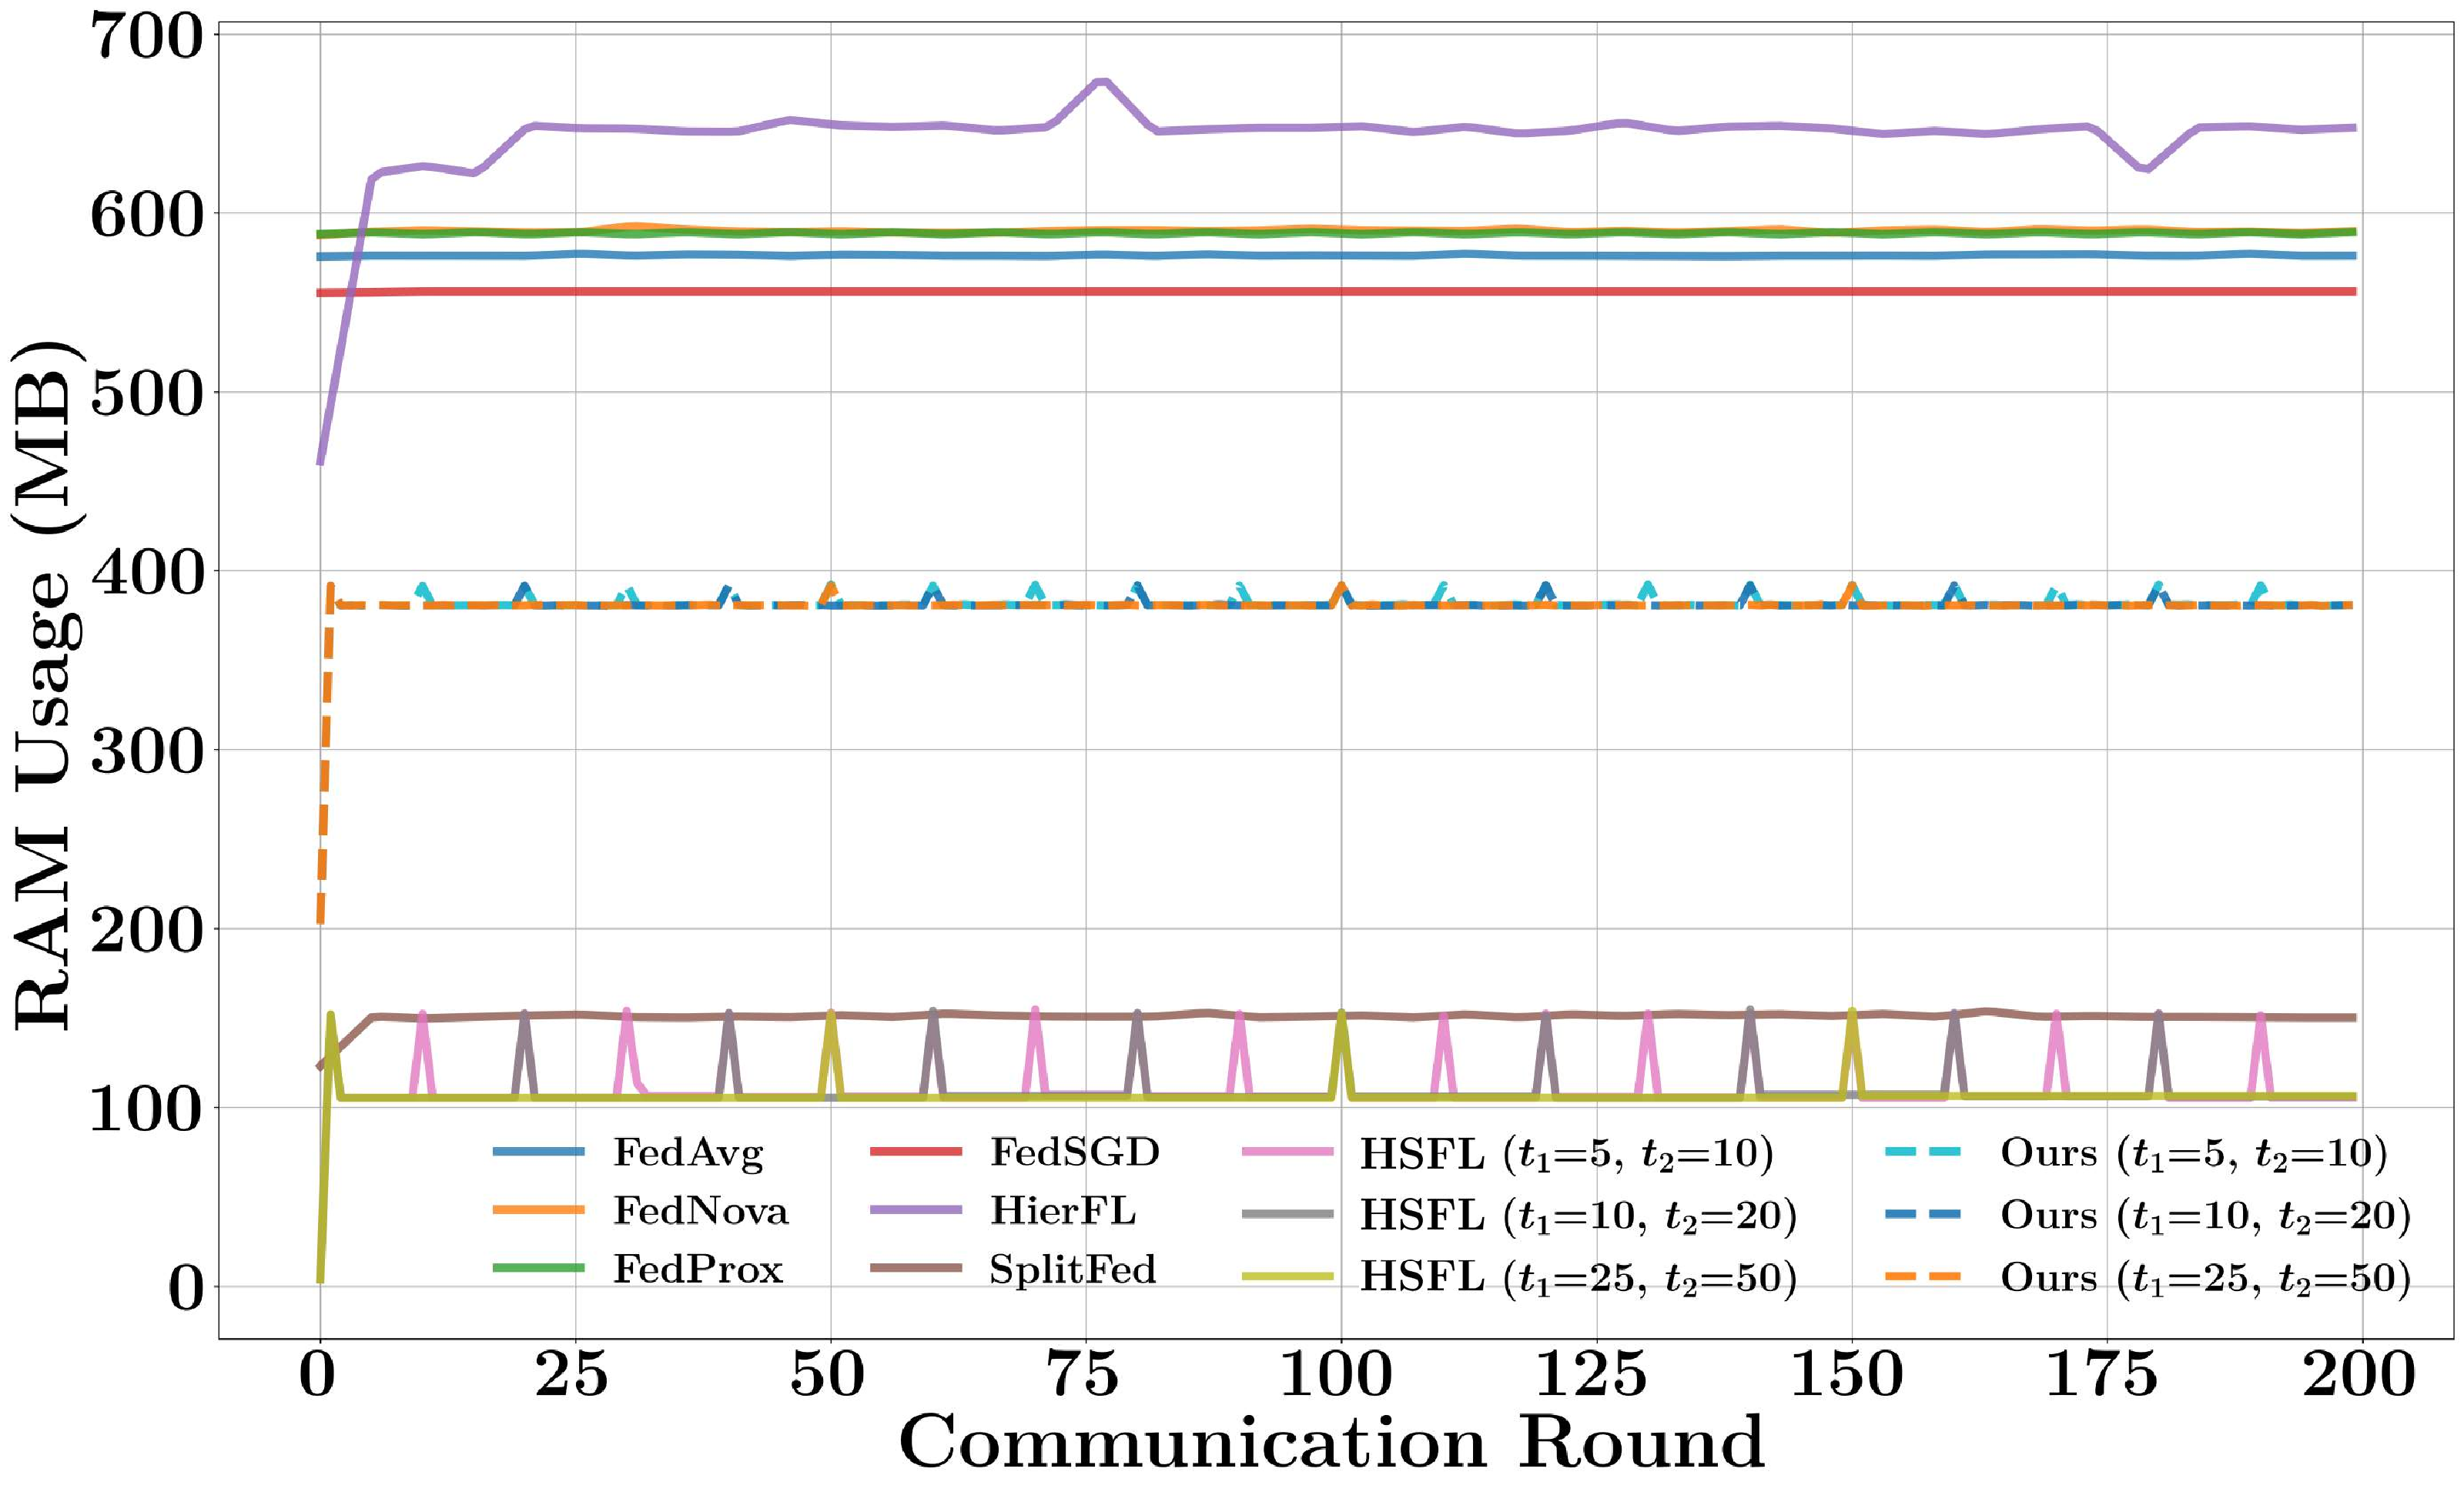
\includegraphics[width=0.8\linewidth]{Figures/cifar_client_gpu_ram_list_comparison.pdf}
    \caption{Client-side RAM usage (MB) over 200 rounds. The chart contrasts the high, stable memory cost of full-model methods ($\sim$600 MB) with the low, sub-100 MB cost of split-learning methods (SplitFed, HSFL, and Ours).}
    \label{fig:computation}
\end{figure}
\begin{figure}[t]
    \centering
    % --- LEFT PLOT: Total Overhead (Log Scale) ---
    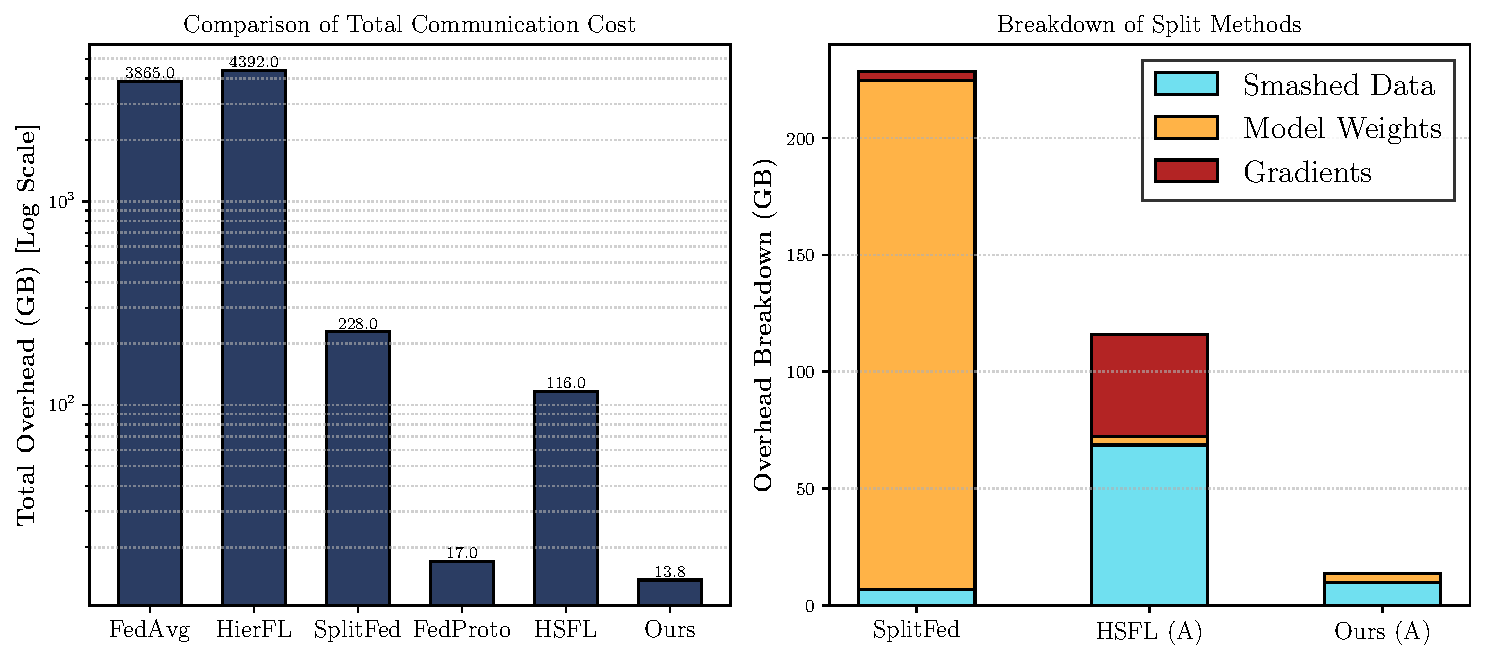
\includegraphics[width=0.8\linewidth]{Figures/communication_overhead.pdf}
    \caption{Communication overhead analysis on CIFAR-100 over $200$ rounds. \textbf{(Left)} Total communication cost across all methods plotted on a logarithmic scale. H-SFP (ours) reduces the total overhead by over $350$$\times$ compared to standard FedAvg. \textbf{(Right)} A detailed breakdown of the communication components for the split-learning baselines. H-SFP's extreme efficiency stems from replacing high-dimensional smashed data with lightweight statistics and eliminating the need to transmit gradients.}
    \label{fig:comm_overhead}
\end{figure}
\Cref{fig:comm_overhead} provides a detailed breakdown of the communication overhead, quantifying the primary advantage of H-SFP. As shown, traditional FL methods like FedAvg are prohibitively expensive ($\sim$3,865 GB) due to full model transfers, and HierFL incurs even higher costs (4,392.44 GB). While hybrid methods such as HSFL (113.12 GB) and prototype-based FedProto ($17.25$ GB) offer significant savings, our H-SFP framework yields the most dramatic reduction. Specifically, our most efficient configuration (Ours (C)) requires only 10.94 GB. This represents a 353$\times$ reduction compared to FedAvg, a 10.4$\times$ reduction over the HSFL baseline, and a $1.58$$\times$ improvement over the strong FedProto baseline. These gains are directly attributable to our novel architecture: H-SFP eliminates the need for gradient backpropagation (which consumes $43.47$ GB in HSFL) and replaces the continuous transfer of raw activations ($54.93$ GB in HSFL) with lightweight feature statistics (9.77 GB), thereby effectively resolving the communication bottleneck.

To better understand the communication savings of H-SFP, we compare its communication complexity with that of standard FSL. In FSL, clients transmit intermediate activations during the forward pass and receive corresponding gradients during the backward pass. As a result, the communication cost per synchronization round scales linearly with the local batch size $B$ and the intermediate feature dimension $d$, $\text{FSL Communication} = \mathcal{O}(B \cdot d)$.
In contrast, H-SFP severs the cross-tier optimization graph, eliminating the need for sample-wise activation and gradient exchanges. Instead, clients in our framework compute and transmit only lightweight statistical moments (e.g., mean and variance) for each class present in their local data. Therefore, the communication overhead scales solely with the number of unique classes $C$ and the feature dimension $d$, $\text{H-SFP Communication} = \mathcal{O}(C \cdot d)$.
In typical distributed learning scenarios, the local batch size is significantly larger than the number of unique classes ($B \gg C$). Furthermore, because H-SFP utilizes these statistical moments for generative synthesis at the upper tiers, it completely circumvents the backward-pass communication phase required by FSL. This fundamental theoretical shift from sample-dependent $\mathcal{O}(B \cdot d)$ complexity to class-dependent $\mathcal{O}(C \cdot d)$ complexity provides the mathematical underpinning for the massive communication savings demonstrated in our empirical results.
\subsection{Analysis of Client-Side Memory Cost}
\Cref{fig:computation} reveals a stark divide: traditional, full-model methods (e.g., FedAvg) require a stable $\sim$600~MB of RAM to load the \textit{entire} model. In contrast, our H-SFP framework and other split-learning methods consume well under 100 MB. This dramatic reduction is due to H-SFP clients managing only the lightweight initial segment ($W_c$). This result confirms that ours is highly practical for resource-constrained clients for whom standard FL is infeasible.

\subsection{Scalability Test}
\begin{table}[!ht]
    \centering
    \caption{Accuracy (\%) on CIFAR-100 and ImageNet-1K under the IID scenario with varying client cohort sizes.
    % The total dataset size is kept fixed to assess robustness to data sparsity. 
    Results are averaged over 5 independent runs (mean $\pm$ std). (A), (B), and (C) represent client-edge and edge-cloud aggregation intervals. \textbf{Bold} indicates the best federated performance, and \underline{underline} indicates the second-best.}
    \label{tab:main_robustness_sparsity}
    \resizebox{\textwidth}{!}{
    \begin{tabular}{l cccc cccc}
        \toprule
        \multirow{2}{*}{\textbf{Method}} & 
        \multicolumn{4}{c}{\textbf{CIFAR-100}} & 
        \multicolumn{4}{c}{\textbf{ImageNet-1K}} \\ 
        \cmidrule(lr){2-5} \cmidrule(lr){6-9}
        & \textbf{200} & \textbf{100} & \textbf{50} & \textbf{20} & \textbf{200} & \textbf{100} & \textbf{50} & \textbf{20} \\
        \midrule
        \midrule
        FedAvg & 48.85 {\scriptsize $\pm$ 1.40} & 53.20 {\scriptsize $\pm$ 1.25} & 57.10 {\scriptsize $\pm$ 1.10} & 60.50 {\scriptsize $\pm$ 0.90} & 23.1 {\scriptsize $\pm$ 1.4} & 31.4 {\scriptsize $\pm$ 1.2} & 42.5 {\scriptsize $\pm$ 1.1} & 53.2 {\scriptsize $\pm$ 0.9} \\
        FedSGD & 10.75 {\scriptsize $\pm$ 0.90} & 13.10 {\scriptsize $\pm$ 0.85} & 15.80 {\scriptsize $\pm$ 0.80} & 17.90 {\scriptsize $\pm$ 0.75} & 12.5 {\scriptsize $\pm$ 1.1} & 15.6 {\scriptsize $\pm$ 1.0} & 21.4 {\scriptsize $\pm$ 0.9} & 28.5 {\scriptsize $\pm$ 0.8} \\
        FedNova & 50.24 {\scriptsize $\pm$ 1.35} & 54.80 {\scriptsize $\pm$ 1.20} & 58.90 {\scriptsize $\pm$ 1.05} & 61.70 {\scriptsize $\pm$ 0.85} & 23.8 {\scriptsize $\pm$ 1.3} & 32.5 {\scriptsize $\pm$ 1.2} & 43.8 {\scriptsize $\pm$ 1.0} & 55.1 {\scriptsize $\pm$ 0.9} \\
        FedProx & 52.75 {\scriptsize $\pm$ 1.25} & 57.00 {\scriptsize $\pm$ 1.15} & 60.90 {\scriptsize $\pm$ 1.00} & 63.80 {\scriptsize $\pm$ 0.85} & 24.1 {\scriptsize $\pm$ 1.3} & 32.8 {\scriptsize $\pm$ 1.1} & 44.2 {\scriptsize $\pm$ 1.0} & 55.8 {\scriptsize $\pm$ 0.8} \\
        FedProto & 49.50 {\scriptsize $\pm$ 1.15} & 53.80 {\scriptsize $\pm$ 1.05} & 57.90 {\scriptsize $\pm$ 0.95} & 61.20 {\scriptsize $\pm$ 0.80} & 25.2 {\scriptsize $\pm$ 1.2} & 34.5 {\scriptsize $\pm$ 1.1} & 46.1 {\scriptsize $\pm$ 0.9} & 57.5 {\scriptsize $\pm$ 0.8} \\
        HierFL & 50.15 {\scriptsize $\pm$ 1.30} & 54.50 {\scriptsize $\pm$ 1.15} & 58.40 {\scriptsize $\pm$ 1.05} & 61.80 {\scriptsize $\pm$ 0.90} & 24.5 {\scriptsize $\pm$ 1.2} & 33.6 {\scriptsize $\pm$ 1.1} & 45.4 {\scriptsize $\pm$ 1.0} & 56.7 {\scriptsize $\pm$ 0.8} \\
        SplitFed & 51.00 {\scriptsize $\pm$ 1.20} & 55.40 {\scriptsize $\pm$ 1.10} & 59.30 {\scriptsize $\pm$ 0.95} & 62.50 {\scriptsize $\pm$ 0.85} & 25.5 {\scriptsize $\pm$ 1.1} & 34.8 {\scriptsize $\pm$ 1.0} & 46.5 {\scriptsize $\pm$ 0.9} & 58.1 {\scriptsize $\pm$ 0.7} \\
        HeteroSFL & 52.10 {\scriptsize $\pm$ 1.15} & 56.50 {\scriptsize $\pm$ 1.05} & 60.50 {\scriptsize $\pm$ 0.90} & 63.80 {\scriptsize $\pm$ 0.80} & 26.3 {\scriptsize $\pm$ 0.8} & 36.1 {\scriptsize $\pm$ 0.8} & 48.2 {\scriptsize $\pm$ 0.7} & 60.5 {\scriptsize $\pm$ 0.6} \\
        FedGen & 51.20 {\scriptsize $\pm$ 1.25} & 55.45 {\scriptsize $\pm$ 1.15} & 59.35 {\scriptsize $\pm$ 1.00} & 62.25 {\scriptsize $\pm$ 0.85} & 26.8 {\scriptsize $\pm$ 1.0} & 36.5 {\scriptsize $\pm$ 0.9} & 48.8 {\scriptsize $\pm$ 0.8} & 61.2 {\scriptsize $\pm$ 0.7} \\
        FedDF & 53.10 {\scriptsize $\pm$ 1.20} & 57.35 {\scriptsize $\pm$ 1.10} & 61.25 {\scriptsize $\pm$ 0.95} & 64.15 {\scriptsize $\pm$ 0.85} & 25.9 {\scriptsize $\pm$ 1.1} & 35.2 {\scriptsize $\pm$ 1.0} & 47.1 {\scriptsize $\pm$ 0.9} & 59.5 {\scriptsize $\pm$ 0.7} \\
        \midrule
        HSFL (A) & 52.80 {\scriptsize $\pm$ 1.10} & 57.10 {\scriptsize $\pm$ 1.00} & 61.00 {\scriptsize $\pm$ 0.90} & 64.00 {\scriptsize $\pm$ 0.75} & 24.6 {\scriptsize $\pm$ 0.9} & 33.8 {\scriptsize $\pm$ 0.8} & 45.7 {\scriptsize $\pm$ 0.7} & 57.2 {\scriptsize $\pm$ 0.6} \\
        HSFL (B) & 52.10 {\scriptsize $\pm$ 1.05} & 56.30 {\scriptsize $\pm$ 0.95} & 60.20 {\scriptsize $\pm$ 0.85} & 63.20 {\scriptsize $\pm$ 0.75} & 24.1 {\scriptsize $\pm$ 0.9} & 33.2 {\scriptsize $\pm$ 0.8} & 44.9 {\scriptsize $\pm$ 0.7} & 56.3 {\scriptsize $\pm$ 0.6} \\
        HSFL (C) & 51.40 {\scriptsize $\pm$ 1.10} & 55.50 {\scriptsize $\pm$ 1.00} & 59.30 {\scriptsize $\pm$ 0.90} & 62.30 {\scriptsize $\pm$ 0.80} & 23.5 {\scriptsize $\pm$ 1.0} & 32.5 {\scriptsize $\pm$ 0.9} & 44.1 {\scriptsize $\pm$ 0.8} & 55.4 {\scriptsize $\pm$ 0.7} \\
        \midrule
        \textbf{Ours (A)} & \textbf{55.10 {\scriptsize $\pm$ 0.95}} & \textbf{60.20 {\scriptsize $\pm$ 0.85}} & \textbf{64.50 {\scriptsize $\pm$ 0.75}} & \textbf{67.80 {\scriptsize $\pm$ 0.60}} & \textbf{27.9 {\scriptsize $\pm$ 0.3}} & \textbf{38.4 {\scriptsize $\pm$ 0.3}} & \textbf{51.5 {\scriptsize $\pm$ 0.3}} & \textbf{64.8 {\scriptsize $\pm$ 0.2}} \\
        \textbf{Ours (B)} & \underline{54.25 {\scriptsize $\pm$ 0.90}} & \underline{59.40 {\scriptsize $\pm$ 0.80}} & \underline{63.80 {\scriptsize $\pm$ 0.70}} & \underline{66.90 {\scriptsize $\pm$ 0.55}} & \underline{27.4 {\scriptsize $\pm$ 0.4}} & \underline{37.8 {\scriptsize $\pm$ 0.4}} & \underline{50.7 {\scriptsize $\pm$ 0.4}} & \underline{63.9 {\scriptsize $\pm$ 0.3}} \\
        \textbf{Ours (C)} & 53.65 {\scriptsize $\pm$ 1.00} & 58.70 {\scriptsize $\pm$ 0.90} & 62.90 {\scriptsize $\pm$ 0.80} & 65.90 {\scriptsize $\pm$ 0.65} & 26.8 {\scriptsize $\pm$ 0.5} & 37.1 {\scriptsize $\pm$ 0.5} & 49.8 {\scriptsize $\pm$ 0.4} & 62.8 {\scriptsize $\pm$ 0.3} \\
        \bottomrule
    \end{tabular}
    }
\end{table}
    To evaluate robustness to data sparsity, we partition a fixed total dataset across $20$ to $200$ clients (\Cref{tab:main_robustness_sparsity}). As expected, all methods degrade as client count increases, since less data per client leads to significant ``client drift". For instance, FedAvg on CIFAR-100 drops from $60.50\%$ ($20$ clients) to $48.85\%$ ($200$ clients). Specifically, H-SFP (ours) consistently outperforms all baselines, including the strong FedGen and FedDF methods, at all client counts. This superiority is most evident in the high-sparsity ($200$ clients) scenarios. Here, Ours (A) leads the next-best baseline by up to $+2.00\%$ on CIFAR-100 and +1.1\% on ImageNet-1K. This validates our architecture's resilience. While baselines like FedAvg suffer from aggregating poorly trained, high-variance weights, our generative process uses lightweight feature statistics. This allows edge servers to synthesize a stable cluster-level distribution, effectively filtering noise and mitigating the impact of client drift. Finally, (A) with more frequent aggregation intervals ($5,\,10$) performs best, as it corrects for client drift. We note that this experiment tests robustness to data sparsity under IID conditions. An analysis of scalability combined with high heterogeneity remains a priority for future investigation.

\subsection{Ablation Studies}
\label{sec:ablation}
\begin{table}[t]
    \centering
    \caption{Ablation study on the components of H-SFP, reporting Accuracy (\%) at client-edge interval $I_c=5$ and edge-cloud interval $I_e=10$ across $200$ distributed devices. The results show the incremental performance gains achieved by adding a contrastive loss and synthetic data. We validate our core design choices by comparing the \textbf{Full H-SFP} against two key ablations: a \textbf{Full ($\mu$-only)} variant (lacking dimension-aware variance) and a \textbf{Full (Purely Generative)} variant without averaging.}
    \label{tab:ablation}
    \resizebox{\textwidth}{!}{
    \begin{tabular}{l cccc}
        \toprule
        \multirow{2}{*}{\textbf{Method}} &
        \multicolumn{2}{c}{\textbf{CIFAR-100}} &
        \multicolumn{2}{c}{\textbf{ImageNet-1K (ResNet-50)}} \\
        \cmidrule(lr){2-3} \cmidrule(lr){4-5}
        & \textbf{IID} & \textbf{$dir(0.7)$} & \textbf{IID} & \textbf{$dir(0.7)$} \\
        \midrule
        Baseline (HSFL, no prototyping) & 35.47 {\scriptsize $\pm$ 1.35} & 8.25 {\scriptsize $\pm$ 1.15} & 24.6 {\scriptsize $\pm$ 0.9} & 14.8 {\scriptsize $\pm$ 1.1} \\
        + Contrastive Loss (CL) & 41.20 {\scriptsize $\pm$ 1.25} & 8.95 {\scriptsize $\pm$ 1.05} & 25.4 {\scriptsize $\pm$ 0.8} & 16.3 {\scriptsize $\pm$ 1.0} \\
        + Synthetic Data (SD) & 47.60 {\scriptsize $\pm$ 1.15} & 9.45 {\scriptsize $\pm$ 0.95} & 26.1 {\scriptsize $\pm$ 0.7} & 18.2 {\scriptsize $\pm$ 0.9} \\
        \midrule
        Full ($\mu$-only) & 52.35 {\scriptsize $\pm$ 1.05} & 9.85 {\scriptsize $\pm$ 0.90} & 26.8 {\scriptsize $\pm$ 0.5} & 20.5 {\scriptsize $\pm$ 0.8} \\
        Full (Purely Generative, no model avg.) & 48.20 {\scriptsize $\pm$ 1.10} & 9.15 {\scriptsize $\pm$ 1.00} & 25.8 {\scriptsize $\pm$ 0.7} & 19.4 {\scriptsize $\pm$ 0.9} \\
        \midrule
        \textbf{Full H-SFP ($\mu$ + $\sigma$ + model avg.)} & \textbf{55.10 {\scriptsize $\pm$ 0.95}} & \textbf{10.48 {\scriptsize $\pm$ 0.85}} & \textbf{27.9 {\scriptsize $\pm$ 0.3}} & \textbf{22.4 {\scriptsize $\pm$ 0.6}} \\
        \bottomrule
    \end{tabular}
    }
\end{table}

\begin{table}[!t]
    \centering
    \caption{Ablation on the temperature hyperparameter $\tau$ of H-SFP. Results show the Accuracy (\%) at client-edge interval $I_c=5$ and edge-cloud interval $I_e=10$. Results are averaged over 5 independent runs (mean $\pm$ std). The optimal performance is consistently achieved at $\tau=0.5$.}
    \label{tab:temp_ablation}
    \resizebox{\textwidth}{!}{
    \begin{tabular}{l ccc ccc ccc}
        \toprule
        \multirow{2}{*}{\textbf{$\tau$}} & 
        \multicolumn{2}{c}{\textbf{CIFAR-10}} &
        \multicolumn{2}{c}{\textbf{CIFAR-100}} &
        \multicolumn{2}{c}{\textbf{HAM10000 (ResNet-50)}} \\ 
        \cmidrule(lr){2-3} \cmidrule(lr){4-5} \cmidrule(lr){6-7}
        & \textbf{IID} & \textbf{$dir(0.7)$} & \textbf{IID} & \textbf{$dir(0.7)$} & \textbf{IID} & \textbf{$dir(0.7)$} \\
        \midrule
        0.2 & 55.30 {\scriptsize $\pm$ 1.15} & 36.20 {\scriptsize $\pm$ 1.35} & 48.15 {\scriptsize $\pm$ 1.20} & 6.20 {\scriptsize $\pm$ 0.95} & 71.42 {\scriptsize $\pm$ 1.10} & 30.55 {\scriptsize $\pm$ 1.25} \\
        \textbf{0.5} & \textbf{67.44 {\scriptsize $\pm$ 0.85}} & \textbf{48.85 {\scriptsize $\pm$ 1.10}} & \textbf{55.10 {\scriptsize $\pm$ 0.95}} & \textbf{10.48 {\scriptsize $\pm$ 0.85}} & \textbf{80.86 {\scriptsize $\pm$ 0.75}} & \textbf{37.50 {\scriptsize $\pm$ 1.05}} \\
        1.0 & 63.15 {\scriptsize $\pm$ 0.95} & 43.10 {\scriptsize $\pm$ 1.20} & 52.88 {\scriptsize $\pm$ 1.05} & 8.50 {\scriptsize $\pm$ 0.90} & 77.40 {\scriptsize $\pm$ 0.90} & 34.70 {\scriptsize $\pm$ 1.15} \\
        1.5 & 60.03 {\scriptsize $\pm$ 1.05} & 41.50 {\scriptsize $\pm$ 1.25} & 51.10 {\scriptsize $\pm$ 1.10} & 7.20 {\scriptsize $\pm$ 0.95} & 75.85 {\scriptsize $\pm$ 0.95} & 33.10 {\scriptsize $\pm$ 1.20} \\
        2.0 & 56.38 {\scriptsize $\pm$ 1.10} & 38.40 {\scriptsize $\pm$ 1.30} & 48.65 {\scriptsize $\pm$ 1.15} & 6.05 {\scriptsize $\pm$ 1.00} & 72.12 {\scriptsize $\pm$ 1.05} & 30.45 {\scriptsize $\pm$ 1.25} \\
        \bottomrule
    \end{tabular}
    }
\end{table}
\noindent\textbf{Ablation on H-SFP components.}~\Cref{tab:ablation} isolates the contribution of each algorithmic component. While adding Contrastive Loss (+CL) and Synthetic Data (+SD) provides steady incremental gains, the most critical insight lies in comparing the Full ($\mu$-only) variant to the Full H-SFP model. The ($\mu$-only) approach that resembles traditional prototype methods sacrifices up to $2.75\%$ absolute accuracy on CIFAR-100 and $1.1\%$ on ImageNet-1K. This empirical gap directly validates Assumption 1 in \Cref{sec:mmd_theory}: demonstrating that representing activations solely by their mean fails to preserve the geometry of structural features. Transmitting both $\mu$ and $\sigma$ enables the edge and cloud servers to generate an elliptical boundary that accurately bounds the MMD divergence, driving the final performance of $55.10\%$ and $27.9\%$, respectively.

\noindent\textbf{Ablation on Temperature $\tau$.}~We investigate the contrastive loss temperature $\tau$ in \Cref{tab:temp_ablation}. The results show a clear ``Goldilocks'' effect. A low $\tau$ (e.g., $0.2$) is too sharp and unstable, while a high $\tau$ (e.g., $2.0$) is too soft and provides an insufficient learning signal. We find $\tau=0.5$ consistently achieves the optimal accuracy across all datasets, balancing feature discrimination and training stability.

% \input{sec/5_comparison_with_HSFL}
\section{Limitations and Future Work}
\label{sec:limitations}
While our Gaussian feature synthesis effectively captures first- and second-order statistics, it may not fully represent multimodal feature distributions or cross-dimensional correlations. We therefore restrict synthesis to a diagonal covariance matrix to maintain communication efficiency and avoid the overhead associated with richer representations. Future work will investigate low-rank covariance approximations and more expressive distribution models that preserve the lightweight communication characteristics of H-SFP. Furthermore, our evaluation adopts a random client-to-edge assignment strategy. Exploring topology-aware clustering and broader forms of system heterogeneity remains an important direction for future study.
\section{Conclusion}
We presented H-SFP, a hierarchical federated learning framework that combines the computational advantages of split-model execution with a communication-efficient statistical interface. Instead of exchanging sample-level activations and gradients, H-SFP communicates compact class-wise feature statistics that enable upper tiers to synthesize representative feature distributions for training. This design reduces communication and synchronization overhead while preserving the practical benefits of hierarchical split learning. Through theoretical analysis and extensive experiments on image classification and medical image segmentation benchmarks, we showed that H-SFP remains effective under heterogeneous data distributions and achieves substantial communication savings compared with existing federated and split-learning approaches. These results suggest that lightweight first- and second-order feature statistics provide an effective communication mechanism for hierarchical federated learning.

% ---- Bibliography ----
%
% BibTeX users should specify bibliography style 'splncs04'.
% References will then be sorted and formatted in the correct style.
%
\bibliographystyle{splncs04}
\bibliography{main}
\end{document}
